\frame{
  \frametitle{Tutte}
\framesubtitle{Tutte's theorem}    
  \begin{figure}[H]
    \centering
    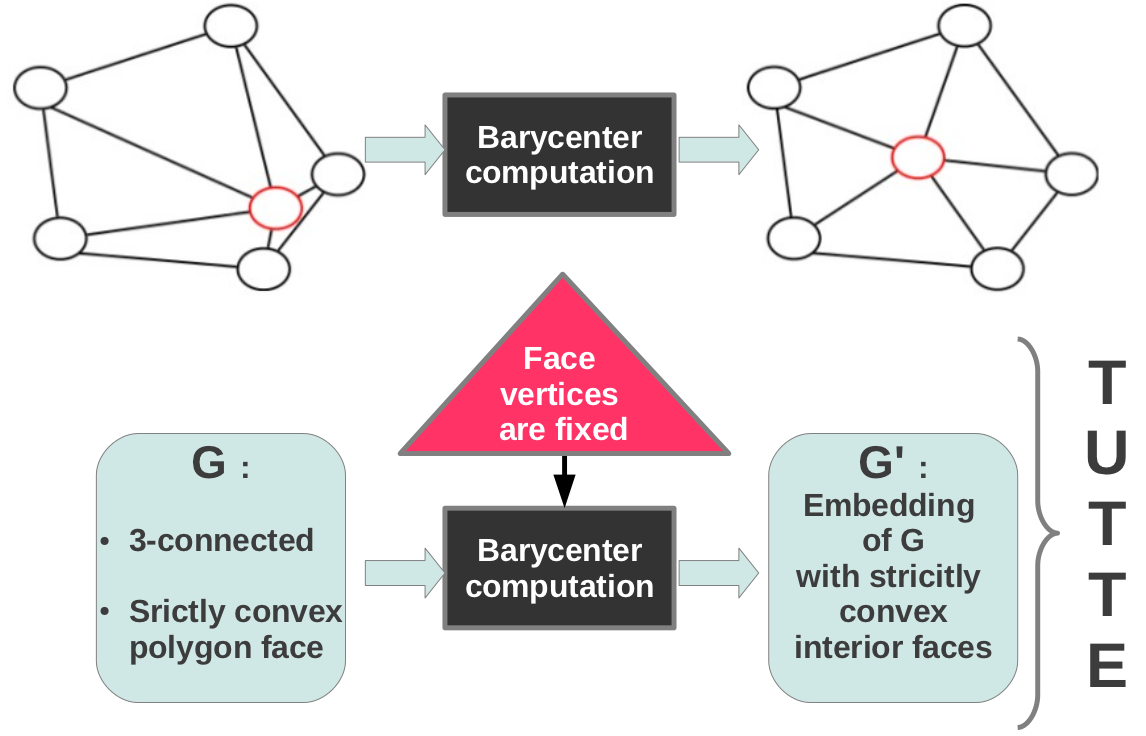
\includegraphics[scale=0.29]{../rapport/img/tutte.png}
  \end{figure}
} 

\frame{
  \frametitle{Tutte}
\framesubtitle{Tutte's theorem}
\begin{columns}[!ht]
\vspace{1cm}
    \begin{column}{6cm}
    \begin{center}
    3-connected graph 
    \end{center}
    \begin{figure}[H]
        \centering
        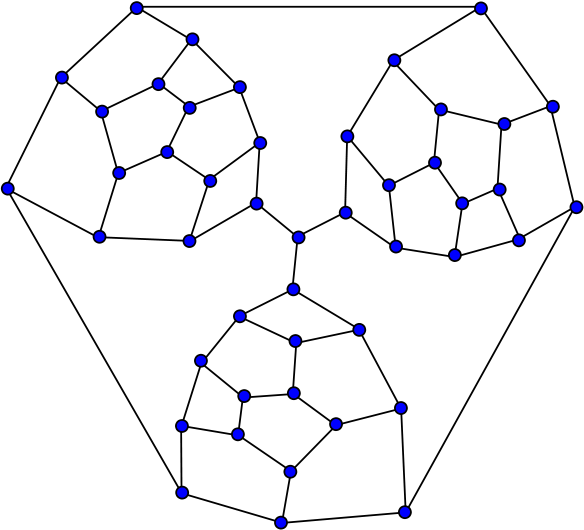
\includegraphics[scale=0.3]{../rapport/img/tutte_graph.png}
      \end{figure}
    \end{column}
    \begin{column}{6cm}
    \begin{center}  
    Tiangle graph
    \end{center}       
      \begin{figure}[H]
        \centering
        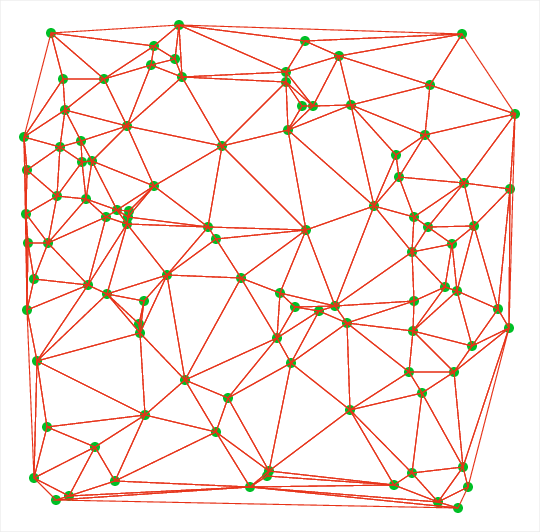
\includegraphics[scale=0.3]{../rapport/img/graph_triangle.png}
      \end{figure}
    \end{column}
  \end{columns}    
}

\frame{
  \frametitle{Tutte}
  \framesubtitle{Tutte's theorem and polygone concave face}
\begin{figure}[H]
    \centering
    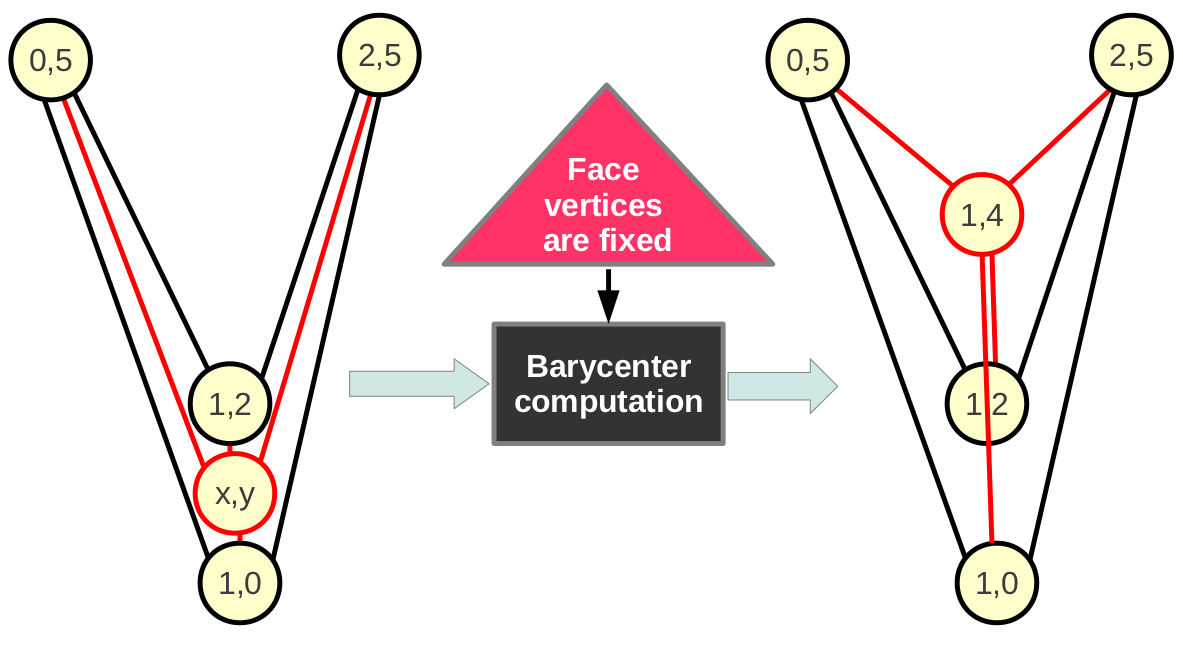
\includegraphics[scale=0.29]{../rapport/img/tutte2.png}
  \end{figure}
} 

\frame{
  \frametitle{Tutte}
\framesubtitle{Tutte's theorem and fixed vertices}
\begin{figure}[H]
    \centering
    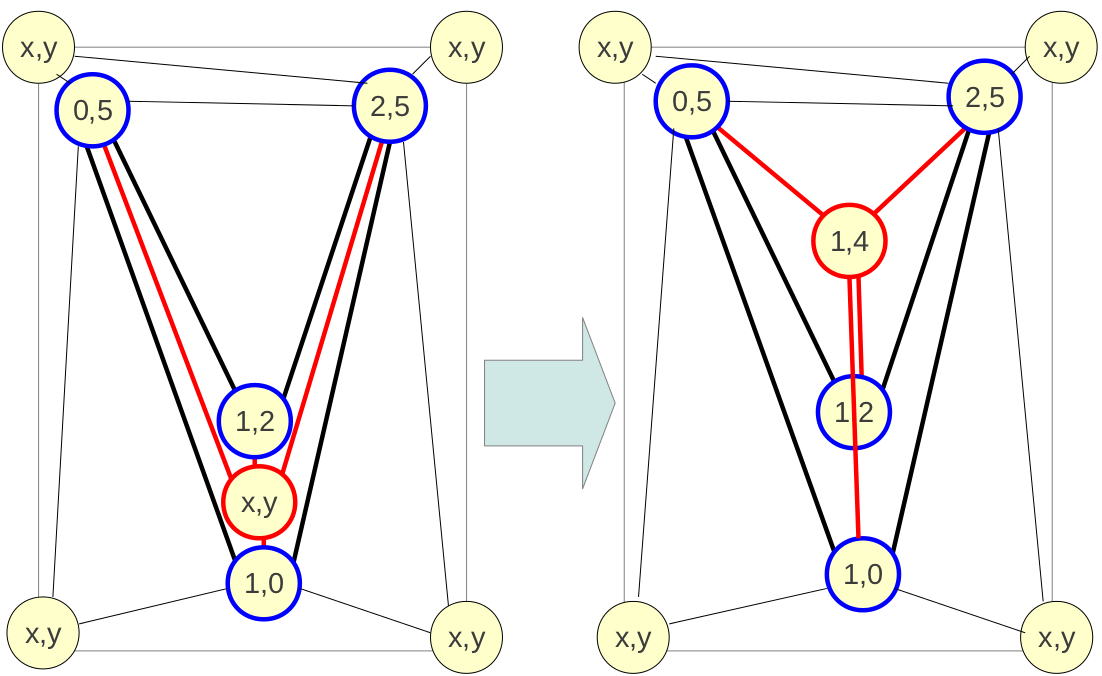
\includegraphics[scale=0.29]{../rapport/img/tutte3.png}
  \end{figure}


} 
